\documentclass{beamer}
\usepackage{amsmath, amssymb, amsthm,tikz,enumerate,listings,url, multimedia}
\usepackage{epsfig,graphics,graphicx,amssymb,amsmath,natbib}%,upmath}
\usepackage[sfdefault=cmbr]{isomath}
\usepackage{color, colortbl,booktabs}
\definecolor{Gray}{gray}{0.9}
\newcommand{\tcr}{\textcolor{red}}
\newcommand{\tcb}{\textcolor{blue}}
\DeclareMathOperator{\arccot}{arccot}
\urlstyle{same}
\setbeamersize{text margin left=10mm, text margin right=10mm}
\usepackage{natbib}
%\newcommand{\newblock}{}

\title{Reflections on Lorentz\\or\\Some new integral equations for surface tractions in Stokes flow}
\author{William Mitchell \& Saverio Spagnolie}
\institute{Mathematics\\ University of Wisconsin - Madison}
\date{APS-DFD, November 2015}

\def\t{\tensorsym}
\newcommand{\bm}{\boldsymbol}
\newcommand{\nv}{^{-1}}
\newcommand{\ds}{\displaystyle}
\newcommand{\mc}[1]{\ensuremath{\mathcal{#1}}}
\newcommand{\ra}{\rightarrow}

\begin{document}
 \begin{frame}
\vspace{-0.3in}\titlepage
\vspace{-0.45in}\begin{center} 
\includegraphics[width=0.4\linewidth]{uwcrest.pdf}\end{center}
\end{frame}

\begin{frame}
\frametitle{Surface tractions}
Problem: determine surface tractions on boundaries in Stokes flow.
\begin{center}
\begin{minipage}{0.5\linewidth}
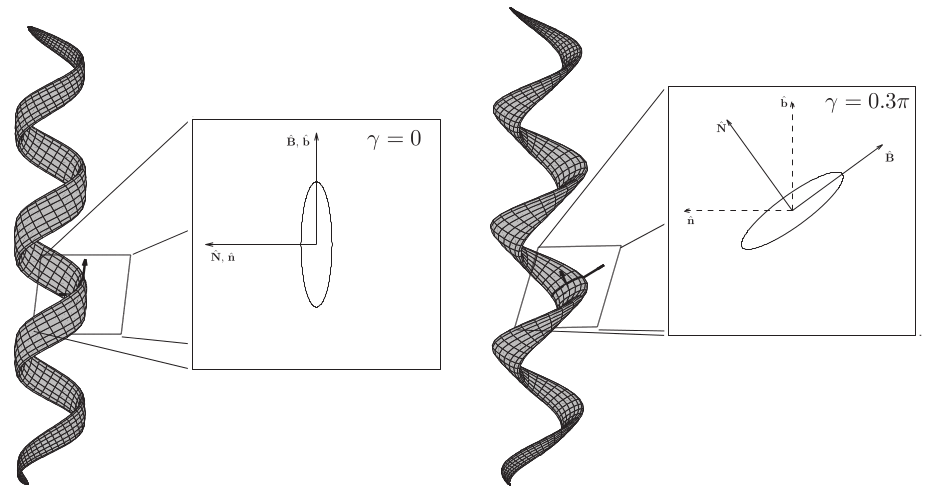
\includegraphics[width = \linewidth]{Spirals.png}
\\
\end{minipage}
% \qquad \qquad
% \begin{minipage}{0.15\linewidth}
% \includegraphics[width = \linewidth]{Blood.jpg}
% \end{minipage}
\end{center}
Options:
\begin{itemize}
 \item $\bm \sigma = \bm I p + \mu (\bm\nabla\bm u + \bm \nabla \bm u ^T)$
 \item Traction integral equations
\end{itemize}
{\footnotesize Shelley \& Keaveny 2011, \emph{Applying a second-kind boundary integral equation
for surface tractions in Stokes flow}}
\end{frame}


\begin{frame}
\frametitle{Integral equations for surface tractions: \only<2>{new cases}}
quiescent\;\;\begin{minipage}{0.3\linewidth}
\begin{center}
free\\
\includegraphics[width = \linewidth]{RCsquare0.pdf}  
\end{center}
\end{minipage}
\quad
\only<2>{
\begin{minipage}{0.3\linewidth}
\begin{center}
wall\\
\includegraphics[width = \linewidth]{RCsquare2.pdf}  
\end{center}
\end{minipage}
\\
\hspace{0.26in}shear\;\;\begin{minipage}{0.3\linewidth}
\includegraphics[width = \linewidth]{RCsquare1.pdf} 
\end{minipage}
\quad
\begin{minipage}{0.3\linewidth}
\includegraphics[width = \linewidth]{RCsquare3.pdf} 
\end{minipage}\\}

\only<1>{
\begin{minipage}{0.4\linewidth}
Shelley \& Keaveny 2011\\
\ \\
Karrila \& Kim 1989\\
Liron \& Barta 1992\\
Kim \& Power 1993\\
Ingber \& Mondy 1993\\
Ladyzhenskaya 1963
\end{minipage}
\qquad 
 \begin{minipage}{0.5\linewidth}
  Goal: 
  \begin{itemize}
   \item simple 
   \item well-conditioned
   \item general
  \end{itemize}
 \end{minipage}
}

\end{frame}
% 
% \begin{frame}
% \frametitle{Extension to background flows: setup} 
% Define:
% \begin{itemize}
%  \item $D$, particle surface
%  \item $B$, large bounding sphere
%  \item $\bm u^\infty$, background flow
%  \item $\bm u,f$: velocity, traction from rigid motion of $D$
%  \item $\bm U, \bm F$ defined through arbitrary $\bm \psi$ on $D$, 
% \[\bm U(\bm x) = \int_D \bm\psi(\bm y)\cdot T(\bm x,\bm y)\cdot \bm n(\bm y)dS_{\bm y} 
% \quad + \int_D C(\bm x,\bm y)\cdot\bm\psi(\bm y)dS_{\bm y} \]  
%  \end{itemize}
% Lorentz Reciprocal theorem gives 
% 
% \end{frame}
% 



\begin{frame}
\frametitle{Accounting for a background flow}
% \hspace{-0.3in}\fbox{\begin{minipage}{0.47\linewidth}
% \begin{center}
% Flow 1: $(\bm u, \sigma)$\\
% rigid particle, background flow\\
% $\bm u = \bm U + \bm\Omega\times\bm x$ on $D$\\
% $|\bm u - \bm u^\infty| = \mathcal{O}(1/r)$
% \end{center}
% \end{minipage}
% }
% \fbox{
% \begin{minipage}{0.5\linewidth}
% \begin{center}
% Flow 2: $(\bm u', \sigma')$\\
% arbitrary $\bm \psi$ on $D$\\
% $\bm u'(\bm x) = \int_D \bm\psi(\bm y)\cdot T(\bm x,\bm y)\cdot \bm n(\bm y)dS_{\bm y} $\\
% $\quad + \int_D C(\bm x,\bm y)\cdot\bm\psi(\bm y)dS_{\bm y} $
% \end{center}
% \end{minipage}
% }
\begin{center}
\begin{itemize}
 \item $(\bm u,\bm f)$ desired flow, decaying to $\bm u^\infty$
\item $(\bm U,\bm F)$ an arbitrary flow via $\bm \psi$ on $D$
 \end{itemize}
 \ \\
Lorentz Reciprocal Theorem\\
$\Downarrow$\\
$\langle \bm u,\bm F \rangle_D +\langle \bm u,\bm F \rangle_B = \langle \bm U,\bm f \rangle_D +\langle \bm U,\bm f \rangle_B$\\
\begin{minipage}{0.3\linewidth}
\includegraphics[width = \linewidth]{LRTBD.pdf} 
\end{minipage}
\begin{minipage}{0.65\linewidth}
\begin{itemize}
\item write all integrals as $\langle\bm \psi, \cdot\rangle$  
\item from $\langle\bm \psi, \mathcal{F}\rangle \equiv 0$ deduce $\mathcal{F} = 0$
\end{itemize} 
\end{minipage}
S\&K (2011) used $\bm u^\infty = \bm 0$
\end{center}
\end{frame}

\begin{frame}

\begin{center}
\begin{minipage}{0.3\linewidth}
\includegraphics[width = \linewidth]{Circ.pdf} 
\end{minipage}
\begin{minipage}{0.2\linewidth}
 $\not \to 0$  
\end{minipage}
\end{center}
\vspace{1in}
but you can calculate it
\end{frame}



\begin{frame}
 \frametitle{Background flows touch the right-hand side only}
\only<1>{For quiet fluid, $\bm u^\infty = \bm0$:}
\only<2>{For simple shear, \textcolor{blue}{$u_i^\infty = \gamma x_3 \delta_{i1}$:}}
\begin{gather}
\begin{split}
\nonumber 
%&\frac{1}{2\eta}f_j(\bm y) + n_k(\bm y)\int_DT_{ijk}(\bm y'-\bm y)f_i(\bm y')dS_{\bm y'} + \int_D C_{ij}(\bm y',\bm y)f_i(\bm y')dS_{\bm y'} \\
&\frac{1}{2\eta}f_j(\bm y) + \int_D K_{ij}(\bm y',\bm y)f_i(\bm y') dS_{y'} = U_j + \epsilon_{jk\ell}\Omega_ky_\ell 
\\
&\quad\only<2>{\textcolor{blue}{+\frac{\gamma}{2}\left[\delta_{1j}y_3-\delta_{3j}y_1\right]
 +\gamma\left[\delta_{1j}n_3(\bm y) + \delta_{3j}n_1(\bm y)\right]}}
%&\quad\only<2>{\textcolor{blue}{- \int_B f_i^\infty(\bm x)\left[ T_{ijk}(\bm x-\bm y)n_k(\bm y) + C_{ij}(\bm x,\bm y)\right]dS_{\bm x}} }\\
%&\quad\only<2>{\;\textcolor{blue}{ +\mu\int_B u_i^\infty(\bm x){\hat n}_m(\bm x)\left[T^{STR}_{ijkm}(\bm x-\bm y)n_k(\bm y) + C^{STR}_{ijm}(\bm x,\bm y) \right]dS_{\bm x} }}
 \end{split}
% \pause
\end{gather}
% \textcolor{blue}{simple shear} ($u_i^\infty = \gamma x_3 \delta_{i1}$):
% \begin{gather}
% \nonumber
% \end{gather}
\end{frame}

\begin{frame}
\frametitle{Application: erosion problem with background shear}

\begin{center}
\begin{minipage}{0.45\linewidth}
Side View\\
\movie[loop]{\includegraphics[width=\linewidth]{CloudStart.jpg}}{Cloud.mpg} 
\end{minipage}
\quad
\begin{minipage}{0.45\linewidth}
Front View\\
\movie[loop]{\includegraphics[width=\linewidth]{FrontViewStart.jpg}}{FrontView.mpg} 
\end{minipage}
\end{center}
% 
% \begin{center}
% \movie{\includegraphics[width=0.4\linewidth]{CloudStart.jpg}}{Cloud.mpg}\\ 
% surface ablation rate $\propto$ shear stress
% \end{center}
c.f.  Ristroph et al. (2012) at high $Re$.  \\
\includegraphics[width = 0.4\linewidth]{High_Re.png}
\end{frame}

\begin{frame}
\frametitle{Next, wall effects}
Replace free-space singularities with wall-bounded counterparts\\
\begin{minipage}{0.3\linewidth}
\includegraphics[width = \linewidth]{Stresslet.pdf} 
\end{minipage}
\quad\begin{minipage}{0.05\linewidth}
 $\to$
\end{minipage}\quad
\begin{minipage}{0.3\linewidth}
 \includegraphics[width =\linewidth]{SStressletImage.pdf}
\end{minipage}
\\
Recompute integrals over $B$
\\
Beware: different singularity subtraction!  $\bm T(\bm x,\bm y) \neq -\bm T(\bm y,\bm x)$
\end{frame}


\begin{frame}
\frametitle{Wall induces torque on translating bodies}
\begin{center}
\movie[loop]{\includegraphics[width=0.45\linewidth]{NSCStart.png}}{NCS.mpg} \;
\movie[loop]{\includegraphics[width=0.45\linewidth]{ProlateStart.png}}{Prolate_Wall_Traction.mpg} 
\end{center}
The net torques on these bodies are opposite in sign! 
\begin{minipage}{0.4\linewidth}
 \includegraphics[width = \linewidth]{Versus.png}
\end{minipage}
\quad
\begin{minipage}{0.5\linewidth}
\begin{itemize}
 \item sphere wants to roll
 \item prolate body wants to glance
\end{itemize} 
\end{minipage}
\end{frame}

% \begin{frame}
% \begin{center}
% \movie{\includegraphics[width=0.45\linewidth]{TO4.png}}{OG.mpg} \;
% \movie{\includegraphics[width=0.45\linewidth]{TO4.png}}{OR.mpg} 
% \end{center}
%  
% \end{frame}

\begin{frame}
\frametitle{Sedimentation of spheroids with wall}
\begin{minipage}{0.45\linewidth}
\begin{center}
3D Oblate Reversing\\
\movie[loop, poster]{\includegraphics[width = \linewidth]{TO4.png}}{OG.mpg}  \\
$\dot y$ changes sign
\end{center}
\end{minipage}
\;
\begin{minipage}{0.45\linewidth}
\begin{center}
3D Oblate Glancing\\
\movie[loop]{\includegraphics[width= \linewidth]{TO4.png}}{OR.mpg} \\
$\dot y < 0$ 
\end{center}
\end{minipage}\\
\ \\
\begin{itemize}
 \item Stokes PDE $\to$ three ODEs governing trajectory
 \item analytical results predict trajectories
\end{itemize}
{\footnotesize Mitchell \& Spagnolie, \emph{Sedimentation of spheroidal particles near walls in viscous fluids: glancing, reversing, tumbling, and sliding.}  JFM 2015}

\end{frame}

\begin{frame}
 \frametitle{Wall \& Shear together}
\begin{minipage}{0.45\linewidth}
\begin{center}
\includegraphics[width= \linewidth]{RCsquare3.pdf}\\
\end{center}
\end{minipage}
\begin{minipage}{0.45\linewidth}
\begin{center}
\includegraphics[width= \linewidth]{ShearWallEllipse.png}\\
\end{center}
\end{minipage}\\
\end{frame}


% 
% 
% \begin{frame}
% \frametitle{Green's functions for Stokes flow are useful tools} 
% \[
% -\bm\nabla p(\bm x) + \mu\nabla^2\bm u(\bm x) = \bm f \delta(\bm x) 
% \]\\
% \[\includegraphics[width = 0.3\linewidth]{StokesletFree.pdf} \]
% \end{frame}

\begin{frame}
\frametitle{History: cancelling Green's functions on a plane wall} 
\textcolor{blue}{Lorentz 1898: General formula for all image flows}\\
\ \\
\textcolor{blue}{$\star$} Blake 1971: singular Green's functions \\
Ainley et al. 2008: regularized Green's functions (special blob only)\\
Cortez et al. 2015: regularized Green's functions (arbitrary blob)\\
Greengard et al. 2015: singular Green's functions
\\\ \\

\end{frame}

\begin{frame}
\frametitle{Lorentz's reflection theorem is simple and powerful}
Suppose that $\bm 0 = -\nabla p + \mu \nabla^2 \bm u$.  \\
Let $\bm \beta$ denote reflection through the plane $\{z = 0\}$.  Define:
\begin{gather}
\label{eq:uhatdef} \bm v = -\bm\beta \bm u - 2z\bm \nabla u_3+z^2 \nabla^2 \bm u\\
\label{eq:phatdef} q = p + 2z\partial_{x_3} p - 4\partial_{x_3} u_3\\
\nonumber \ \\
\label{eq:ustardef} \bm u^*(x,y,z) = \bm \beta \bm v(x,y,-z)\\
\label{eq:pstardef} p^*(x,y,z) = q(x,y,-z)
\end{gather}
Then $\bm u + \bm u^* = \bm 0$ on $\{z = 0\}$ and $\bm 0 = -\bm\nabla(p+p^*) + \mu\nabla^2(\bm u+\bm u^*)$.  
\end{frame}


\begin{frame}
\frametitle{The LRT Stresslet image is concise}
\begin{center}
\(\displaystyle T_{ijk}(\bm x,\bm y) = \frac{\hat X_i \hat X_j\hat X_k}{|\hat X|^5}\)\\
\alt<1>{\includegraphics[width = 0.3\linewidth]{Xhatdef.pdf} }{\includegraphics[width = 0.3\linewidth]{XhatXdef.pdf}}
\includegraphics[width = 0.3\linewidth]{Stresslet.pdf} 
\pause
{\includegraphics[width = 0.3\linewidth]{SStressletImage.pdf} 
\vspace{-0.2in}
{\small
\begin{align*}
&\hspace{-0.35in} T^*_{ijk}(\bm x,\bm y) = -\frac{\hat X_iX_jX_k}{|\bm X|^5} - 2x_3\frac{\beta_{ij}y_3X_k+\beta_{ik}y_3X_j-\delta_{jk}x_3\beta_{im}X_m}{|\bm  X|^5} + 10\frac{x_3y_3X_jX_k\beta_{im}X_m}{|\bm  X|^7}
\end{align*}
}
}
\end{center}
\end{frame}

% 
% \begin{frame}
% \frametitle{Future work}
% \begin{itemize}
%  \item Shear flow past a bump on a wall
% % \begin{minipage}{0.4\linewidth}
% % \includegraphics[width = \linewidth]{RCsquare3.pdf} 
% % \end{minipage}
% % \quad$\to$\quad
% \begin{minipage}{0.4\linewidth}
% \includegraphics[width = \linewidth]{RCsquare4.pdf} 
% \end{minipage}
%  \item Forced background flows, $-\bm\nabla p + \mu\nabla^2\bm u \neq 0$
%  \item Several bodies
% \item $\star$ Rigid-body restriction? $\star$
%  \end{itemize}
% \end{frame}


\begin{frame}
\frametitle{Q \& A}
\begin{minipage}{0.3\linewidth}
\begin{center}
\includegraphics[width = \linewidth]{NCSEnd.png}  
\end{center}
\end{minipage}
\quad
\begin{minipage}{0.3\linewidth}
\begin{center}
\includegraphics[width = \linewidth]{CloudEnd.jpg}  
\end{center}
\end{minipage}
\quad
\begin{minipage}{0.3\linewidth}
\begin{center}
\includegraphics[width = \linewidth]{ShearWallEllipse.png}  
\end{center}
\end{minipage}\\
\begin{minipage}{0.3\linewidth}
\includegraphics[width = \linewidth]{RCsquare2.pdf} 
\end{minipage}
\quad
\begin{minipage}{0.3\linewidth}
\includegraphics[width = \linewidth]{RCsquare1.pdf} 
\end{minipage}
\quad
\begin{minipage}{0.3\linewidth}
\includegraphics[width = \linewidth]{RCsquare3.pdf} 
\end{minipage}
\end{frame}



\end{document}
